\chapter{绪论}
\section{研究背景和意义}
优秀的开放域对话机器人(聊天机器人)应该有娱乐性和知识,同时让用户觉得自己能够被倾听。可能的谈话主题的广度和缺乏一个明确的目标使得很难定义一个培训优秀聊天机器人的路线图。尽管最近学术界和工业界在这方面取得了全面进展~\cite{adiwardana2020meena,roller2020recipes},但聊天机器人仍然无法在进行对话的同时保持有趣、一致、准确和可靠,以及在谈论各种话题时保持行为端正(例如,不冒犯用户)。

传统的面向任务的对话系统依赖于槽填充和结构化模块(例如,\citet{young2013pomdp,gao2019neural,jurafsky2019speech}),这些方法已经证明擅长在飞机票预订等狭窄领域开发可用的商业系统。然而,它们仅限于接受培训的领域,无法推广到新领域或开放聊天设置,因为这需要对许多模块或技能进行编码,以及在它们之间切换的管理系统。另一方面,基于神经网络的端到端的方法提供了适应任意宽的新领域而无需额外人工的可能,但尚未达到其全部潜力。端到端训练的深度架构在许多其他领域都非常成功,例如语音识别~\cite{hinton2012deep,collobert2016wav2letter}, 计算机视觉~\cite{krizhevsky2012imagenet},和机器翻译~\cite{sutskever2014sequence,gehring2017convolutional}。因此,研究界正在大力投资改进对话的端到端模型~\cite{zhang2019dialogpt,adiwardana2020meena,roller2020recipes},希望取得类似的成功。为了提升用户的体验,聊天机器人需要具备一些关键的对话理解能力,比如,聊天机器人应该识别说话者情感,能够理解对话语义,以及能够理解并正确处理对话中的不安全行为。

\textbf{情感}是人类固有的,因此情感理解是人工智能的关键部分。对话情绪识别作为自然语言处理的重要研究方向,由于具有挖掘意见的能力,近些年来越来越受欢迎,并且如今在Facebook、Youtube、Reddit、Twitter等平台上有着大量公开可用的对话数据可以用于研究。此外,对话情绪识别对于产生情感意识的对话也很重要。为了满足这些需求,需要有效和可扩展的对话情绪识别算法。

\textbf{对话语义}是说话者意图表达的核心载体,理解对话语义的难点是对话中普遍存在的省略与指代,主要原因是人们为了简洁方便,倾向于使用不完整的话语来对话,这通常会省略或引用出现在对话上下文中的概念。具体来说,\citet{su-etal-2019-improving,pan-etal-2019-improving}指出,省略和指代存在于超过70\%的对话语句中,这会给对话模型带来额外的负担,因为他们必须识别出这些省略和指代才能正确理解对话。对话角色语义标注和对话重写是两个对话语义理解的自然语言处理任务,它们的模型能够帮助聊天机器人更好地理解对话,进而生成更好地与用户进行交谈。

\textbf{安全性}是人工智能的能力越来越强大道路上必须改善的问题。随着在大规模语料库上预训练的基于 transformer 的语言模型的出现,生成式开放域聊天机器人越来越受到关注 \cite{zhang2020dialogpt,wang2020cdialgpt,adiwardana2020meena}。然而,由于对其不可控制和不可预测的输出的安全担忧,生成对话模型在现实世界中的部署仍然受到限制。例如,微软的 TwitterBot \textit{Tay} 于 2016 年发布,但在其种族主义和有毒评论引起公众强烈反对后很快被召回 \cite{micro2016exam}。
直到现在,对话安全仍然是生成对话模型的致命弱点。如何让聊天机器人更好地理解对话中的不安全行为是急需解决的问题。


\section{相关工作}
\subsection{对话情绪识别}
对话情绪识别(Emotion Recognition in Conversation, ERC) 一直是一个NLP领域长期的研究课题~\cite{devillers2002annotation,lee2005toward}。早期工作通过人工的语言或声学特征来解决 ERC ~\cite{devillers2006real,forbes2004predicting}。 随着深度学习模型在分类和序列建模任务中的主导地位不断提高~\cite{poostchi-etal-2018-bilstm,kipf2016semi,vaswani2017attention},
最近的 ERC 研究基于深度学习,深度学习可以进一步分为三种主要类型:基于 RNN 的模型、基于 GCN 的模型和基于 Transformers 的模型。 基于 RNN 的模型在过去几年中得到了很好的探索。 \citet{poria2017context} 首先使用递归神经网络 (RNN) 对 ERC 的对话上下文进行建模~\cite{medsker2001recurrent}。 \citet{hazarika2018conversational} 考虑了说话人的信息,并且 \citet{hazarika2018icon} 首先模拟了说话人之间的依赖关系。 \citet{majumder2019dialoguernn} 跟踪说话者的状态,他们的方法可以扩展到多方对话。 \citet{lu2020iterative} 提出了一种基于 RNN 的迭代情感交互网络来显式建模话语之间的情感交互。 \citet{ghosal2019dialoguegcn} 和 \citet{sheng2020summarize} 采用关系图卷积网络 (GCN)~\cite{schlichtkrull2018modeling} 对 ERC 进行建模,其中整个对话被视为有向图,他们采用图卷积运算来捕获之间的依赖关系顶点(话语)。 但是,将对话转换为图形会丢失原始对话的时间属性。 由于 Transformers \cite{vaswani2017attention} 出色的表征能力,一些研究人员将其应用于 ERC 并取得了良好的结果 \cite{zhong2019knowledge,li2020hitrans}。 最近,\citet{ghosal2020cosmic} 将从预训练的常识转换器 COMET \cite{bosselut2019comet} 中提取的常识知识整合到 RNN 中,并在几个公共 ERC 数据集上获得了良好的结果。然而,上述模型都没有考虑上下文缺失或上下文冗余问题。

\subsection{自训练}
自训练~\cite{scudder1965probability,Angluin1988-yw,Abney2002-qo,lee2013pseudo}是一个经典的半监督学习框架~\cite{chapelle2009semi}近年来被广泛探索。自训练的总体思路是采用训练好的模型对容易获取的未标记数据进行伪标记,并使用它们来扩充训练数据以迭代地重新训练模型。该范式在各种任务中显示出良好的效果:包括文本分类~\cite{mukherjee2020uncertainty,wang2020adaptive}、图像分类~\cite{xie2020self,zoph2020rethinking}、机器翻译~\cite{he2019revisiting} 和模型蒸馏~\cite{mukherjee2020xtremedistil}。协同训练~\cite{blum1998combining} 和三重训练~\cite{zhou2005tri} 是与自训练类似的迭代训练框架,但具有不同数量的模型或考虑训练了数据的不同视图,两者都在 NLP领域得到了广泛采用~\cite{Mihalcea2004-ks,McClosky2006-mp,Wan2009-jq,Li2014-ie,Caragea2015-fm,Lee2021-uj,Wagner2021-qo}。这些框架旨在通过在一项任务上训练多个模型来提高性能,而不会利用相关任务的监督信号。

\subsection{多任务学习}
多任务学习~\cite{caruana1997multitask,yang2021survey}旨在其他相关任务的帮助下提高一个任务的学习性能,其中有两块工作与我们的相关:(1) 半监督多任务学习~\cite{liu2007semi,li2009active}结合了半监督学习和多任务学习。 \citet{liu2007semi} 通过随机游走利用未标记数据,并使用任务聚类方法进行多任务学习。 \citet{li2009active} 将主动学习~\cite{mackay1992information} 与 \citet{liu2007semi} 中的模型相结合,以检索最能提供标签信息的数据。尽管这些工作试图利用未标记的数据来增强多任务学习,但我们的工作与它们的不同之处在于我们通过在任务之间结合监督信号以选择高质量的伪标签来更新模型,这是一个迭代训练过程,无需额外的人工。 (2) 任务分组~\cite{kumar2012learning,standley2020tasks,fifty2021efficiently}旨在找到相关任务组,并对每组任务采用多任务学习,每组一个模型。我们的工作重点是训练单任务模型,但任务分组技术可用于寻找可能的相近任务。

\subsection{对话语义角色标注} 对话角色语义标注(Conversational Semantic Role Labeling, CSRL)是一项预测对话上下文中谓词语义角色的任务。图~\ref{fig:csrl} 显示了一个 3 轮的中文CSRL的例子,其中像“雪宝”是第二轮中第二个谓词“喜欢”的“A1”谓元,这样的关系明确指出了核心的主谓宾关系(也是用“喜欢”来表达的细粒度情绪)。然而,传统的语义角色标注只能作用于一个句子,因此可能无法捕获对话语句之间的关键信息。例如,图~\ref{fig:csrl}中第二个句子中的谓词“看了”的两个谓元“A0”和“AM-TMP”在传统语义角色标注中可能会被漏掉,因为这些谓元是存在于对话中的其他句子的。另外,预测第三个句子中的谓词“喜欢”和“雪宝”之间的关系是很有挑战性的,因为这同时需要知道“它”是“喜欢”的“A1”,以及“它”是“雪宝”的代词(指代消解)。
\begin{figure}[!ht]
\centering
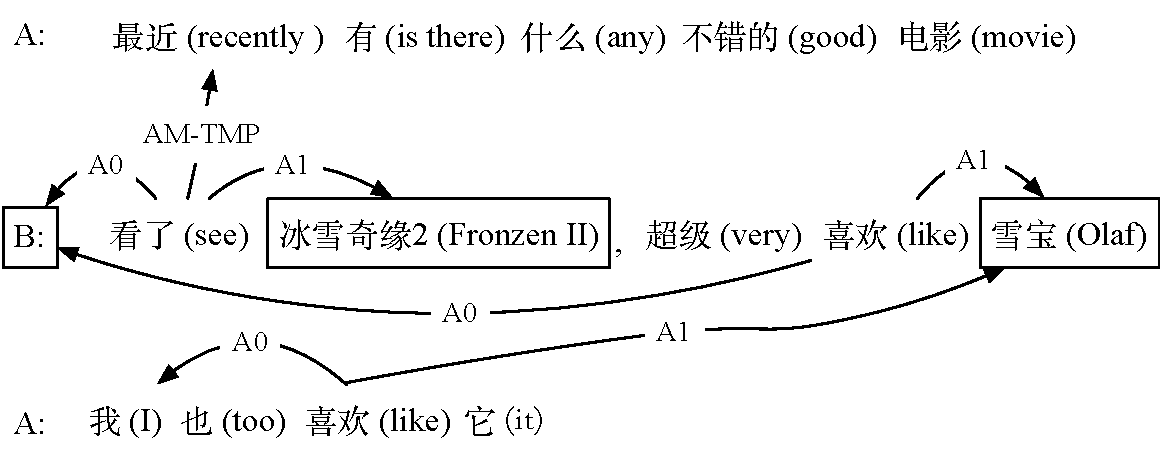
\includegraphics[width=0.8\textwidth]{pics/intro_v2.pdf}
\caption{对语义角色标注的示例。 这个涵盖了所有核心关系,而传统的语义标注只能覆盖用黑色箭头表示的关系。 一条斜线表示共指关系。}\label{fig:csrl}
\end{figure}

\citet{wu2021csagn} 利用关系图神经网络~\cite{schlichtkrull2018modeling}对说话者和谓词依赖性进行建模,取得了一些有希望的结果。 但是,CSRL 的当前数据集 ~\cite{xu2021conversational} 仅限于单域。 需要新领域的高质量标记数据来增强更适用的 CSRL 模型。


\subsection{对话重写} 对话重写~\cite{su-etal-2019-improving,pan-etal-2019-improving,elgohary2019can}旨在将最新的对话话语重构为与原始话语在语义上等同的新话语,并且无需参考上下文即可理解。如表~\ref{tab:example} 所示,不完整的话语 $u_3$ 省略了“上海”,并用代词“这样”引用了“经常阴天下雨”,通过将丢弃的信息显式重写进最新的话语,下游对话模型就只需要采用最后的话语。 这样就可以大大减轻长距离推理的负担。

            
\definecolor{zptu}{RGB}{18, 141, 21}
\newcommand{\zptu}[1]{\textcolor{zptu}{(zptu: #1)}}
\begin{table} \small
    \centering
    \caption{一个对话重写的示例,包括上下文话语($u_1$ 和 $u_2$)、最新话语($u_3$)和重写话语($u_3^\prime$)。}
    \label{tab:example}
    \begin{tabular}{cc}
    \toprule
    Turn & Utterance with Translation \\
    \midrule
    \multirow{2}{*}{$u_1$} & 上海最近天气怎么样?\\
         & (How is the recent weather in Shanghai?) \\
    \midrule
    \multirow{2}{*}{$u_2$} & 最近经常阴天下雨。\\
         & (It is always raining recently.) \\
    \midrule
    \multirow{2}{*}{$u_3$} & 冬天就是\textcolor{blue}{这样}。\\
         & (Winter is like \textcolor{blue}{this}.) \\
    \midrule
    \multirow{2}{*}{$u_3^\prime$} & \textcolor{zptu}{上海}冬天就是\textcolor{blue}{经常阴天下雨}。\\
         & (It is \textcolor{blue}{always raining} in winter \textcolor{zptu}{Shanghai}.) \\
    \bottomrule
    \end{tabular}
    \vspace{-1.2em}
\end{table}

对话重写通常被认为是一个序列到序列的问题,它会遇到很大的搜索空间问题~\cite{elgohary2019can,huang2021sarg}。为了解决这个问题,\citet{hao2021rast} 将对话重写转换为序列标签,将重写话语转换为从话语中删除符号或将对话历史中的跨度插入话语中。 \citet{jin2022hierarchical} 改进了 \cite{hao2021rast} 中的连续跨度问题,首先为每个符号和开槽规则生成多个跨度,然后用跨度替换固定数量的规则。然而,高质量的对话重写训练数据仍然是缺乏的。

\subsection{对话安全数据集} 近年来构建了关于带有不同形式标注的对话安全的数据集。 对于不安全检测,\citet{qian2019benchmark}、\citet{xu2020recipes}、\citet{baheti2021just}、\citet{ung2021saferdialogues} 和 \citet{sun2021safety} 在他们提出的对话数据集中提供了话语级二类安全标签。 \citet{baheti2021just} 注释了同一对话中每个话语的立场(\textit{stance}) 以间接帮助不安全检测。 为了引导对话避免不安全的失败,\citet{qian2019benchmark} 和 \citet{ung2021saferdialogues} 分别从第三方或对话伙伴提供以自然语言表示的干预(\textit{intervention}) 和 反馈(\textit{feedback})来避免话语中不安全的发生。 \citet{ung2021saferdialogues} 进一步要求标注者给出优雅的响应以确认 \textit{feedback} 并将对话引入可接受且文明的轨迹,聊天机器人可以从中学习如何从不安全行为中恢复。 然而,据我们所知,目前还没有带有不安全跨度和上下文相关安全替代响应的的数据集。

\subsection{有毒行为的缓解} 为了检测不安全的内容,基于Transformers~\cite{devlin2018bert,liu2019roberta}的分类器是主要的方法,因为它们具有很强的表示能力,一些数据集~\cite{davidson2017automated,hartvigsen2022toxigen} 可以作为主要资源用于训练强大的毒性检测器。更精细的毒性检测,即提取毒性跨度或短语,可以看作是序列标注~\cite{yang2018design}任务。对于文本去毒,\citet{santos2018fighting} 和 \citet{laugier2021civil} 训练了一个编码器-解码器模型,将有毒话语重写为无毒话语。 \citet{dathathri2019plug} 和 \citet{krause2020gedi} 利用鉴别器来约束语言模型,让它的生成无毒,并且 \citet{dale2021text} 利用转述模型改进了 \citet{krause2020gedi} 的方法。 \citet{ouyang2022training} 和 \citet{glaese2022improving} 通过强化学习注入人类反馈,使生成的响应更有用且无害。

\section{章节和内容安排}
本文共分为五个章节,各章节具体安排如下:

第一章:绪论。本章介绍本文中每个工作的任务背景和意义,并阐述一下与工作相关的有关文献的进展和内容,以及存在的问题。

第二章:基于变长上下文的对话情绪识别。本章提出了一种新的对话情绪分析方法,能够从可变长度的上下文中识别说话者的情绪。本章的实验和消融研究表明,提出的方法可以有效缓解对话情绪分析中的上下文缺失和上下文冗余问题,同时在三个公共数据集上实现具有竞争力的性能。

第三章:基于友邻训练的对话理解。本章提出了友邻训练,这是第一个跨任务自训练框架,它利用友邻任务的监督来更好地选择伪标签。此外,本章在对话语义角色标注和对话重写之间实现了友邻训练。领域泛化和少样本学习场景的实验证明了友邻训练的前景,它大幅度优于之前的经典或最先进的半监督方法。

第四章:基于\data{}的对话不安全行为理解。本章提出了\data{},第一个具有对话安全综合标注的大规模数据集。 \data{} 标注了不安全跨度以回答为什么话语不安全,并提供安全的替代响应来替换不安全的响应来更好地理解对话中的不安全行为。 实验和分析表明,\data{} 有效地推进了对话不安全行为的解释和解毒。

第五章:总结全文并且基于现有的工作给出未来展望。
